\documentclass[12pt]{article}
\usepackage[french]{babel}
\usepackage[utf8]{inputenc}
\usepackage{amsmath}
\usepackage{amssymb}
\usepackage{geometry}
\usepackage{xcolor}
\usepackage{graphicx}
\geometry{a4paper, margin=1in}

\title{DS commun Sujet B}
\author{Lycée Jacques Decour - Seconde 2025-2026}
\date{}

\begin{document}

\maketitle

{\color{red}
\underline{\textbf{(À LIRE) Remarques générales :}}

\vspace{5pt}
\begin{itemize}
    \item Globalement un devoir avec des résultats un peu en dessous que ce dont vous avez l'habitude
    de produire. Ça arrive mais attention car ce DS est important, il porte sur de nombreuses 
    notions à maîtriser pleinement pour la suite du lycée

    \vspace{5pt}
    \item Le barème apparaît ici sur chaque question 
    
    \vspace{5pt}
    \item beaucoup d'erreurs sur l'identité remarquable $(a-b)^2 = a^2 - 2ab + b^2$, vous êtes énormément
    à m'avoir écrit : $a^2 -2a(-b) + b^2$, le signe $-$ n'apparaît \textbf{qu'une seule fois}

    \vspace{5pt}
    \item Je ne le répèterai jamais assez : \textbf{\underline{SIMPLIFIEZ VOS RÉSULTATS ET VOS}}

    \noindent\textbf{\underline{FRACTIONS}}. L'année prochaine on vous enlèvera des points pour ça.
    
    \vspace{5pt}
    \item beaucoup (trop) d'erreurs de calculs avec les \textbf{fractions}, vous êtes nombreux à 
    m'écrire $-2 \times \dfrac{2}{3} = \dfrac{-4}{-6}$ ou encore $\dfrac{-4}{6}$. Ceci est \textbf{FAUX}

    \vspace{5pt}
    \item encore sur les fractions, pour faire $4 \times \dfrac{9}{4}$ on ne fait pas $\dfrac{36}{4}$,
    on simplifie directement les $4$ ! C'est du niveau collège !

    \vspace{5pt}
    \item j'insiste sur le nombre trop grand d'erreurs de calculs littéral ou de développement, ou 
    de factorisation, il faut retravailler tout ça chez vous
\end{itemize}
}

\section*{Exercice 1}

Soit $f$ la fonction définie sur $\mathbb{R}$ par :
\[
f(x) = 4x^2 - 5
\]

\begin{enumerate}
    \item Calculer l'image de $-2$ par la fonction $f$.
    {\color{red} \boxed{11}}

    \item Calculer l'image de $\dfrac{3}{2}$ par la fonction $f$.
    {\color{red} \boxed{4}}

    \item Déterminer les antécédents éventuels de $-13$ par la fonction $f$.
    {\color{red} \boxed{\text{Aucun antécédent réel.}}}
\end{enumerate}

\section*{Exercice 2}

\begin{enumerate}
    \item Déterminer par des lectures graphiques l'expression de la fonction affine $f$ représentée sur la figure 1 par la droite $\mathcal{D}$ :

    \begin{center}
        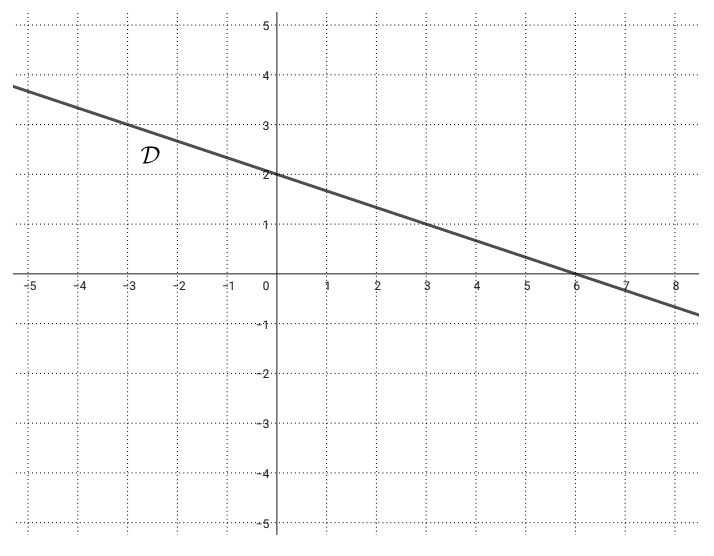
\includegraphics[width=0.8\textwidth]{fig1.png}

        \vspace{-20pt}
        \textbf{FIGURE 1}
    \end{center}

    {\color{red} \boxed{\text{$f(x) = \dfrac{1}{3}x - 4$}}}

    \item Dans le repère de la figure 1, tracer la représentation graphique de la fonction $g$ définie sur $\mathbb{R}$ par $g(x) = -\dfrac{3}{5}x + 2$.

    {\color{red} \boxed{\text{Je vous laisse répondre à cette question par vous-même}}}
\end{enumerate}

\section*{Exercice 3}

On considère deux fonctions $f$ et $g$ définies sur l'intervalle $[-8; 5]$ dont les représentations graphiques sont données sur la figure 2. Répondre aux questions à l'aide de lectures graphiques.

\begin{center}
    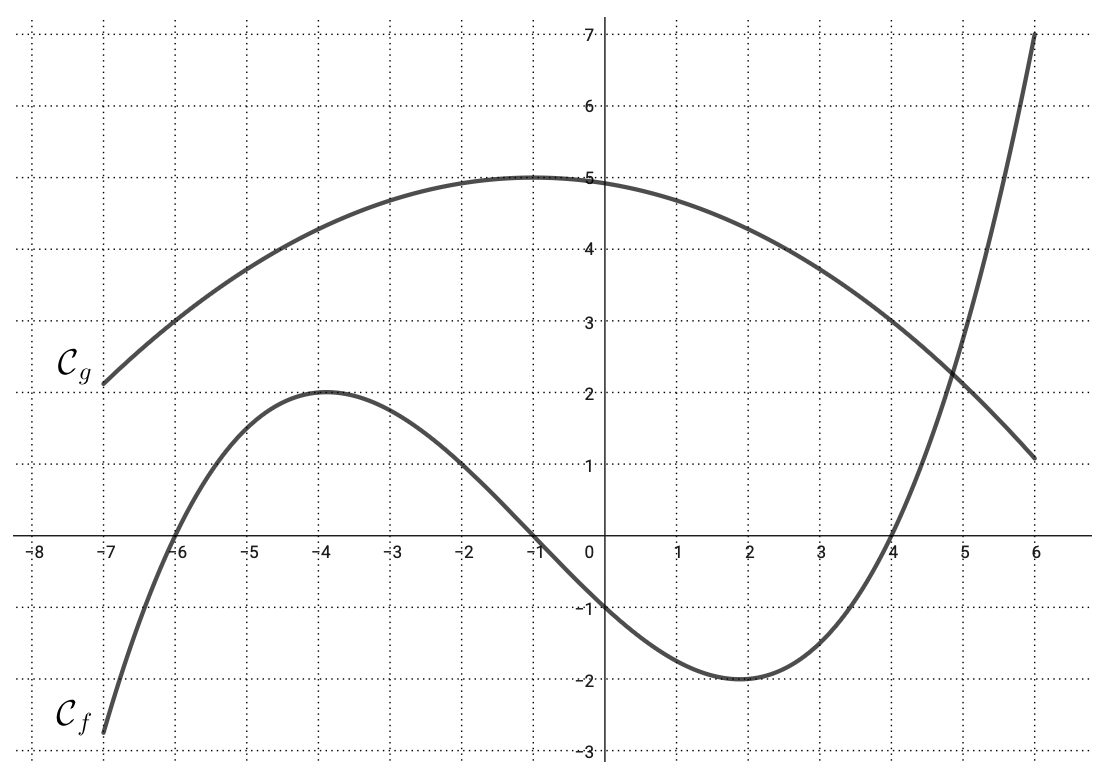
\includegraphics[width=0.8\textwidth]{fig2.png}
    
    \textbf{FIGURE 2}
\end{center}

\begin{enumerate}
    \item Déterminer l'image de $3$ par la fonction $g$. {\color{red} \boxed{\text{environ 4,2}}}
    \item Déterminer les antécédents éventuels de $0$ par la fonction $f$. {\color{red} \boxed{\text{-6 ; -1 et 4}}}
    \item Résoudre l'inéquation : $f(x) \geq 1$. {\color{red} \boxed{\text{$\left[-8;-6,4\right] \cup \left[0 ; 3,5\right]$ à peu près}}}
    \item Résoudre l'inéquation : $f(x) < g(x)$. {\color{red} \boxed{\text{$\left]-6,8;5\right]$}}}
    \item Dresser le tableau de signes de la fonction $f$. 
    
    {\color{red} \boxed{\text{Je vous laisse refaire cette question par vous même.}}}

    \item Dresser le tableau de variations de la fonction $f$. 
    
    {\color{red} \boxed{\text{Je vous laisse refaire cette question par vous même.}}}
\end{enumerate}

\section*{Exercice 4}

\begin{enumerate}
    \item Développer et réduire les expressions suivantes :
    \[
    A = (-4x + 3)(x - 5), \quad B = x - \dfrac{3}{4}(x - 2), \quad C = (5x - 1)^2
    \]
    {\color{red}
    \[
    A = \boxed{-4x^2 + 23x - 15} \quad , \quad B = \boxed{\dfrac{1}{4}x + \dfrac{3}{2}} \quad , \quad C = \boxed{25x^2 - 10x + 1}
    \]}

    \item Factoriser les expressions suivantes :
    \[
    D = 4x^2 - 1, \quad E = 5x^2 - 3x, \quad F = x^2 - 8x + 16
    \]
    {\color{red}
    \[
    D = \boxed{(2x - 1)(2x + 1)} \quad , \quad E = \boxed{x(5x - 3)} \quad , \quad F = \boxed{(x - 4)^2}
    \]}
\end{enumerate}

\section*{Exercice 5}

\begin{enumerate}
    \item Résoudre les équations d'inconnue réelle $x$ :

    \begin{enumerate}
        \item $\dfrac{2}{3}x + 1 = 5$
        {\color{red} \boxed{x = 6}}

        \item $(-2x + 8)(x + 7) = 0$
        {\color{red} \boxed{x = 4 \text{ et } x = -7}}

        \item $x^2 = 10$
        {\color{red} \boxed{x = -\sqrt{10} \text{ et } x = \sqrt{10}}}
    \end{enumerate}

    \item Résoudre les inéquations d'inconnue réelle $x$ :

    \begin{enumerate}
        \item $-3x - 6 \geq x + 2$
        {\color{red} \boxed{x \leq -2 \hspace{1cm} S=]-\infty;-2]}}

        \item $\dfrac{3x + 2}{-2x + 10} \leq 0$
        {\color{red} \boxed{x \in \left]-\infty; -\dfrac{2}{3}\right] \cup \left[5; +\infty\right[}}
    \end{enumerate}
\end{enumerate}

\end{document}